\documentclass[12pt]{article}
\usepackage[english]{babel}
\usepackage{natbib}
\usepackage{url}
\usepackage{hyperref}
\usepackage{minted}
\usepackage{listings}
\usepackage[utf8x]{inputenc}
\usepackage{graphicx}
\graphicspath{{images/}}
\usepackage{fancyhdr}
\usepackage{vmargin}
\setmarginsrb{3 cm}{2.5 cm}{3 cm}{2.5 cm}{1 cm}{1.5 cm}{1 cm}{1.5 cm}
\title{Práctica 2: Bootloader que escribe en la pantalla}% Title 
\author{Meza Madrid Damián}% Author
\date{Febrero 2019}% Date
\makeatletter
\let\thetitle\@title
\let\theauthor\@author
\let\thedate\@date
\def\@seccntformat#1{%
  \expandafter\ifx\csname c@#1\endcsname\c@section\else
  \csname the#1\endcsname\quad
  \fi}
\makeatother
\pagestyle{fancy}
\fancyhf{}
\rhead{\theauthor}
\lhead{\thetitle}
\cfoot{\thepage}
\begin{document}

%%%%%%%%%%%%%%%%%%%%%%%%%%%%%%%%%%%%%%%%%%%%%%%%%%%%%%%%%%%%%%%%%%%%%%%%%%%%%%%%%%%%%%%%%

\begin{titlepage}
	\centering
    \vspace*{0.5 cm}
    
\includegraphics[scale = 0.30]{escom.png}\\[1.0 cm]	% University Logo
	\textsc{\Large Instituto Politécnico Nacional}\\[0.5 cm]% Course Code
	\textsc{\Large Escuela Superior de Computo}\\[0.5 cm]% Course Code
	\rule{\linewidth}{0.2 mm} \\[0.4 cm]
	{ \huge \bfseries \thetitle}\\
	\rule{\linewidth}{0.2 mm} \\[1.5 cm]
	Reporte\\
	Profesor: Ulises Velez Saldaña \\
	Alumno: Meza Madrid Raúl Damián\\
    Clase: Sistemas operativos\\
    Grupo: 2CM7\\
\end{titlepage}
\tableofcontents
\pagebreak
\section{Introducción}
Como se vio en la practica pasada, el boot loader aquel encargado de buscar y cargar el sistema operativo. Durante el proceso de booteo, el control lo tiene primero el BIos, después se lo pasa al boot loader. Una vez en el boot loader es posible llamar interrupciones del BIOs\\
Una \emph{interrupcion} es un mecanismo que tienen las computadoras que detiene el ciclo de fetch para atender un evento solicitado o no solicitado. Se usan para:
\begin{itemize}
    \item Seguridad
    \item Operaciones I/O
    \item Funciones del BIOS y O.S.
\end{itemize}
Esta práctica tiene como propósito utilizar las llamadas a interrupciones del BIOS de diferentes maneras para escribir un mensaje desde el boot loader. Así como utilizar los principios vistos en clase para las direcciones en la que el boot loader debe cargar.
\subsection{Programas y herramientas utilizados}
Esta práctica fue desarrollada en el sistema operativo Ubuntu 18.04.1 LTS. Los programas y herramientas utilizados, junto con el comando de instalación, en caso de que no estuvieran instalados ya. 
\begin{itemize}
    \item NASM : \$ apt-get install nasm
    \item QEMU : \$ apt-get install qemu
    \item dd
    \item genisoimage
\end{itemize}
\section{Objetivo}
Que el alumno aplique la teoría vista en clase, conozca el proceso y las herramientas necesarias para construir el cargador.
\section{Desarrollo}
Para desarrollar y ejecutar la práctica, se debe seguir el procedimiento de la práctica anterior para crear las imágenes tanto de Floppy Disk como CD-ROM\\
Se utilizo el sigueinte script de bash compilar el programa, crear sus respectivas imagenes y montarlo en la máquina virtual.
\begin{minted}{bash}
#!/usr/bin/env bash
nasm src/bootloader.asm -f bin -o bin/bootloader
dd if=/dev/zero of=images/escomOS.flp bs=1024 count=1440
dd if=bin/bootloader of=images/escomOS.flp seek=0 count=1 conv=notrunc
genisoimage -quiet -V 'escomOS' -input-charset iso8859-1 -o ./images/escomOS.iso -b images/escomOS.flp -hide images/escomOS.flp .
qemu-system-i386 -fda images/escomOS.flp
qemu-system-i386 -cdrom images/escomOS.iso

nasm src/bootloaderVidMem.asm -f bin -o bin/bootloadervidMem
dd if=/dev/zero of=images/escomOSVidMem.flp bs=1024 count=1440
dd if=bin/bootloaderVidMem of=images/escomOSVidMem.flp seek=0 count=1 conv=notrunc
genisoimage -quiet -V 'escomOSVidMem' -input-charset iso8859-1 -o ./images/escomOSVidMem.iso -b images/escomOSVidMem.flp -hide images/escomOSVidMem.flp .
qemu-system-i386 -fda images/escomOSVidMem.flp
qemu-system-i386 -cdrom images/escomOSVidMem.iso
\end{minted}
\subsection{Primera parte}
El primero debe utilizar la interrupción 10H del BIOs. Debe considerar que el bootloader es cargado en la dirección 0x07c00(ya sea en el segmento y offset 0000:07C00 o 07C0:0000). Sigue el siguiente proceso:
\begin{itemize}
    \item Mueve DS a 0x07C0 antes de invocar la interrupción del BIOS \cite{BasicBootloader}
    \item Asegúrate de que la bandera de dirección indique de menor a mayor (DF=0) \cite{DF} \cite{cld} \cite{banderas}
    \item Debes investigar como se escribe un carácter con la interrupción 10H \cite{Int10h} \cite{list} \cite{HowtoHello}
    \item Declara una variable con el mensaje que se desea escribir y colocar un cero al final para marcar el fin del mensaje
    \item En un ciclo escribe cada carácter verificando que no haya llegado a cero
\end{itemize}
\subsubsection{Interrupciones tipo 10h a 1Fh} 
Las rutinas de interrupciones 10h a 1Fh pueden ser llamadas por programas para realizar varias operaciones de entrada salida (I/O) o para revisar el estado de la maquina. 
\subsubsection{Interrupción 10h -- Vídeo}
La rutina de interrupción 10h es el driver de vídeo. Esta asociada con cada dispositivo de I/O. Existe un dispositivo o controlador I/O que actúa como interfaz tipo hardware entre el procesador y el dispositivo mismo de I/O. El dispositivo controlador ejecuta varias tareas de bajo nivel especificas al dispositivo de I/O. Esto permite que la CPU interactúe con el dispositivo a un nivel mas alto \cite{Int10h}
\subsubsection{INT 10h / AH = 0Eh - Salida a teletipos.}
Entradas:\\
AL = Carácter a escribir.\\\\
Esta función muestra un carácter en la pantalla, avanzando el cursor y moviendo la pantalla como sea necesario. La escritura siempre es a la pagina activa. \cite{list}
\subsubsection{Programa}
\begin{minted}[breaklines,mathescape,linenos,numbersep=5pt,frame=single,numbersep=5pt,xleftmargin=0pt,]{asm}
; Trabajando en 16 bits
bits 16
start:
; Mover el DS (Direction Segment) a la direccion 17c0
  mov ax, 07c0h
  mov ds, ax
; cld limpia la vandera de direccion (DF=0)
	cld
; Entra en modo TYY
  mov ah, 0Eh
  ;Se declara el mensaje y se guarda la direccion del mismo en SI
	mov si, msg
; Comienza el ciclo, lodsb es para sacar uno por uno los caracteres de SI  a AL
.loop	lodsb
; Compara el contenido en al con un 0
	cmp al, 0
; Si el resultado es verdadero, va a done:
	je done
; Interrupcion para escribir el caracter
	int 10h
; Regresa a loop
	jmp .loop 
; Se declara la cadena con el 0 al final
msg:	db 'Este no es mi primer ni ultimo hola mundo', 0
; Funcion cuando encuentra el fin de la cadena (linea 18)
done:
; Magic Numbers
times 510 - ($ - $$) db 0
dw 0xAA55
\end{minted}
\subsubsection{Resultados}
\begin{figure}[!htb]
\begin{minipage}{0.5\textwidth}
El bootloader ahora muestra nuestro mensaje después del mensaje de 'Booting from ...'
\end{minipage}
\begin{minipage}{0.5\textwidth}
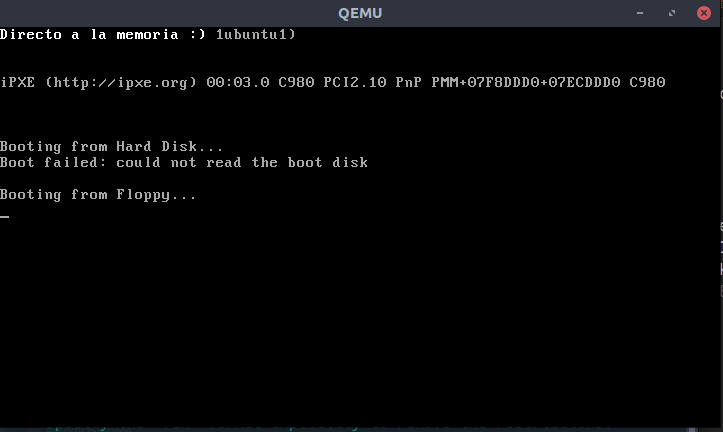
\includegraphics{ParteDos.png}
\end{minipage}
\end{figure}
\subsection{Segunda parte}
El segundo bootloader debe escribir directamente en la memoria de video. Usa como ejemplo el programa anterior y mueve carácter por carácter a la memoria de video. Considera lo siguiente:
\begin{itemize}
    \item Investiga y documenta todo lo que puedas sobre la memoria de video.
    \item Recuerda que cara caracter tiene un atributo en la memoria de video y que la dirección por defecto es B8000.
\end{itemize}
\subsubsection{Memoria de video}
A la hora de escribir en la memoria de video, la cual comienza en 0xb8000, existen dos bytes por cada cuadro o celda en la pantalla. El carácter a mostrar es el primer byte, mientras que el segundo es el atributo del mismo. Para escribir un carácter en la esquina superior izquierda, es necesario mover la palabra formada por \cite{dirMem}
\subsubsection{Programa}
\begin{minted}[breaklines,mathescape,linenos,numbersep=5pt,frame=single,numbersep=5pt,xleftmargin=0pt,]{asm}
; Trabajando en 16 bits
bits 16
start:
; Mover el DS (Direction Segment) a la direccion 17c0
  mov ax, 07c0h
  mov ds, ax
; Se usa el ES (Extra Segment) a la direccion de video
  mov ax,0xb800
  mov es,ax 
;Se declara el mensaje y se guarda la direccion del mismo en SI
  mov si, msg
;Movemos el DI a la direccion para la esquina superior izquierda
  mov di,0x0
; Comienza el ciclo
.loop
  mov al,[si]    ; se carga el byte del caracter
  mov ah,0x0f    ; se carga el byte de la configuracion, fondo negro letra blanca
  mov [es:di],ax ; se carga el registro de al y ah (ax)a la direccion correspondiente
  inc si         ; siguiente caracter
  add di,2       ; se le suma 2 la direccion (1 por el caracter y otro por la configuracion)
  cmp al,0       ; Compara el contenido con un 0
  je done        ; Si es verdadero, se va a done:
  jmp .loop      ; Repite el ciclo

  ; Se declara la cadena con el 0 al final
msg:	db 'Directo a la memoria :)', 0
  ; Funcion cuando encuentra el fin de la cadena (linea 18)
done:
  ; Magic Numbers
  times 510 - ($ - $$) db 0
  dw 0xAA55
\end{minted}
\subsubsection{Resultados}
\begin{figure}[!htb]
\begin{minipage}{0.5\textwidth}
El programa sobre-escribió el texto de la maquina virtual y escribió nuestro mensaje en colores mas brillantes
\end{minipage}
\begin{minipage}{0.5\textwidth}
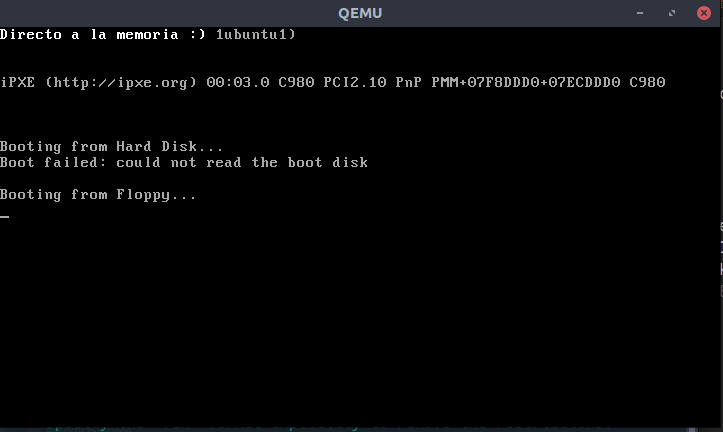
\includegraphics{ParteDos.png}
\end{minipage}
\end{figure}
\subsection{Errores y problemas}
\begin{figure}[!htb]
\begin{minipage}{0.5\textwidth}
El primer error fue que cuando quería dejar el numero 0xb800 de la misma manera en la que escribí 07c0h, , la escribí como b800h pero el programa dejaba de funcionar. Honestamente no me moleste en investigar la razón del problema, así que solo lo cambie de vuelta. \\
El segundo error fue que escribí di cuando iba si era di en la instruccion mov [es:di],ax ; lo cual resulto en muchos caracteres de colores. 
\end{minipage}
\begin{minipage}{0.5\textwidth}
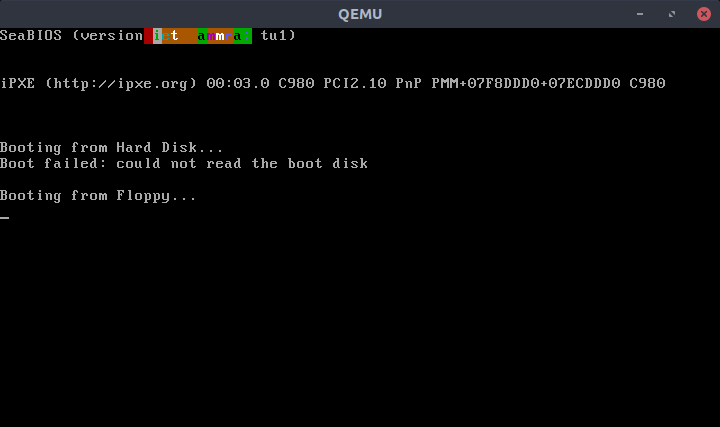
\includegraphics{Prompt.png}
\end{minipage}
\end{figure}
\section{Codigo (Github)}
Todo el codigo de esta practica se puede encontrar en :\url{https://github.com/asdf1234Damian/Operating-Systems/tree/master/Practica02/Proyecto}
\nocite{*}
\addcontentsline{toc}{section}{References}
\bibliographystyle{plain}
\bibliography{biblist}
\end{document}

